% !TEX root =  ../main_manuscript.tex 
\section{Results}
The cause-specific cumulative upgrading-risk at year five of follow-up was 35\% in PRIAS and at most 50\% in validation cohorts (Panel~B, Figure~\ref{c5:fig:4}). In the fitted PRIAS model, the adjusted hazard ratio (aHR) of upgrading for an increase in patient age from 61 to 71 years (25-th to 75-th percentile) was 1.45~(95\%CI:~1.30--1.63). For an increase in fitted PSA value from 2.36 to 3.07 (25-th to 75-th percentile, log scale), the aHR was 0.99~(95\%CI:~0.89--1.11). The strongest predictor of upgrading-risk was instantaneous PSA velocity, with an increase from -0.09 to 0.31 (25-th to 75-th percentile), giving an aHR of 2.47~(95\%CI:~1.93--2.99). The aHR for PSA value and velocity was different in each GAP3 cohort (Table~\ref{c5:tab:PSA_survival_gap3}).

The time-dependent AUC, calibration plot, and time-dependent MAPE of our model are shown in Figure~\ref{c5:fig:4}, and Figure~\ref{c5:fig:auc_pe_recalib}. In all cohorts, time-dependent AUC was moderate (0.6 to 0.7) over the whole follow-up period. Time-dependent MAPE was moderate (0.1 to 0.2) in those cohorts where the impact of PSA on upgrading-risk was similar to PRIAS (e.g., Hopkins cohort, Table~\ref{c5:tab:PSA_survival_gap3}), and large (0.2 to 0.3) otherwise. Our model was miscalibrated for validation cohorts (Panel~B, Figure~\ref{c5:fig:4}), because cohorts had differences in inclusion criteria (e.g., PSA density) and follow-up protocols~\citep{gap3_2018} which were not accounted in our model. Consequently, the PRIAS based model's fitted baseline hazard did not correspond to the baseline hazard in validation cohorts. To solve this problem, we recalibrated the baseline hazard of upgrading in validation cohorts (Figure~\ref{c5:fig:calib_before_after}). We compared risk predictions from the recalibrated models, with predictions from separately fitted cohort-specific joint models (Figure~\ref{c5:fig:calib_in_small}). The difference in predictions was lowest in the Johns Hopkins cohort (impact of PSA on upgrading-risk similar to PRIAS). Comprehensive results are in Appendix~\ref{c5:appendix:full_results} and Appendix~\ref{c5:appendix:validation_res}.

\begin{figure}
\centerline{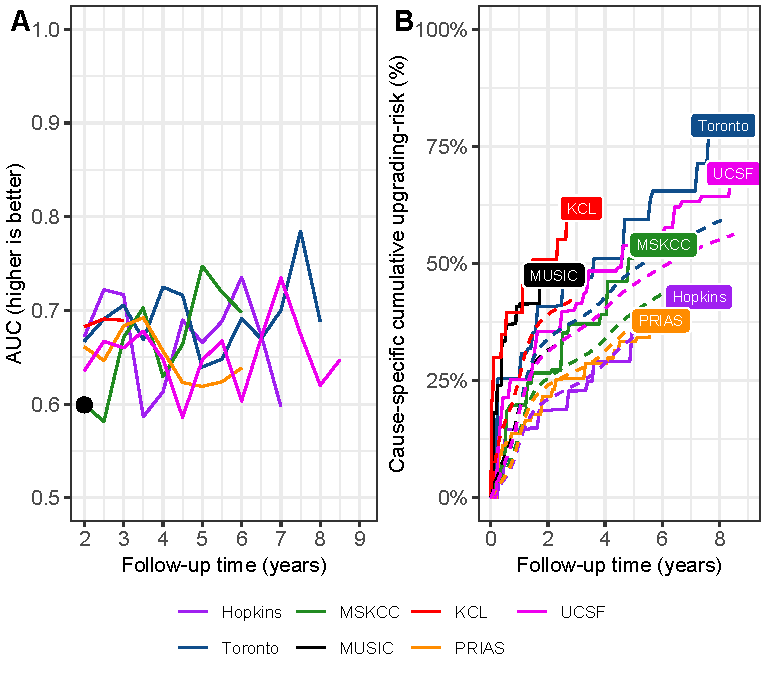
\includegraphics{contents/c5/images/c5_fig4.pdf}}
\caption{\textbf{Model Validation Results}. \textbf{Panel~A}: time-dependent area under the receiver operating characteristic curve or AUC (measure of discrimination). AUC at year one is not shown because we do not intend to replace the confirmatory biopsy at year one. \textbf{Panel~B}: calibration-at-large indicates model miscalibration. This is because solid lines depicting the non-parameteric estimate of the cause-specific cumulative upgrading-risk~\citep{turnbull1976empirical}, and dashed lines showing the average cause-specific cumulative upgrading-risk obtained using the joint model fitted to the PRIAS dataset, are not overlapping. Recalibrating the baseline hazard of upgrading resolved this issue (Figure~\ref{c5:fig:calib_before_after}). Full names of Cohorts are \textit{PRIAS}: Prostate Cancer International Active Surveillance, \textit{Toronto}: University of Toronto Active Surveillance, \textit{Hopkins}: Johns Hopkins Active Surveillance, \textit{MSKCC}: Memorial Sloan Kettering Cancer Center Active Surveillance, \textit{KCL}: King's College London Active Surveillance, \textit{MUSIC}: Michigan Urological Surgery Improvement Collaborative Active Surveillance, \textit{UCSF}: University of California San Francisco AS.}
\label{c5:fig:4}
\end{figure}

\subsection{Personalized Biopsy Schedules}
We employed the PRIAS based fitted model to create personalized biopsy schedules for real PRIAS patients. Particularly, first using the model and patient's observed data, we predicted his cumulative upgrading-risk (Figure~\ref{c5:fig:5}) on all of his future follow-up visits (biannually in PRIAS). Subsequently, we planned biopsies on those future visits where his conditional cumulative upgrading-risk was more than a certain threshold (see Chapter~\ref{c4:sec:schedule} for mathematical details). The choice of this threshold dictates the timing of biopsies in a risk-based personalized schedule. For example, personalized schedules based on 5\% and 10\% risk thresholds are shown in Figure~\ref{c5:fig:5}. 

To facilitate the choice of a risk-threshold, and for comparing the consequences of opting for a risk-based schedule versus any other schedule (e.g., annual, PRIAS), we predict expected time delay in detecting upgrading for following a schedule. We are able to predict this delay for any schedule. For example, in Panel~C of Figure~\ref{c5:fig:5}, the annual schedule has the least expected delay. In contrast, a personalized schedule based on a 10\% risk threshold has a slightly larger expected delay, but it also schedules much fewer biopsies. An important aspect of this delay is that it is personalized as well. That is, even if two different patients are prescribed the same biopsy schedule, their expected delays will be different. This is because delay is estimated using all available clinical data of the patient (Chapter~\ref{c4:subsec:exp_delay_estimation}). While the timing and the total number of planned biopsies denote the burden of a schedule, a shorter expected time delay in detecting upgrading can be a benefit. These two, along with other measures such as a patient's comorbidities, anxiety, etc., can help to make an informed biopsy decision.

\begin{figure}
\centerline{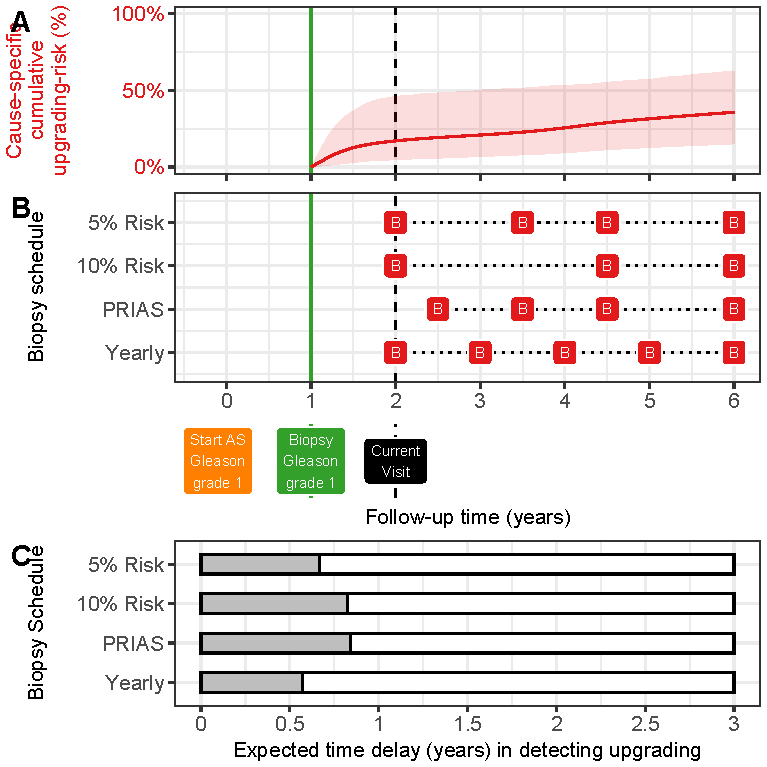
\includegraphics{contents/c5/images/c5_fig5.pdf}}
\caption{\textbf{Illustration of personalized and fixed schedules of biopsies for patient from Figure~\ref{c5:fig:3}}. \textbf{Panel~A:} Predicted cumulative upgrading-risk (95\% credible interval shaded). \textbf{Panel~B:} Different biopsy schedules with a red `B' indicating a future biopsy. Risk:~5\% and Risk:~10\% are personalized schedules in which a biopsy is planned whenever the conditional cause-specific cumulative upgrading-risk is above 5\% or 10\% risk, respectively. Green vertical line at year one is the time of the latest negative biopsy. Black dashed line at year two denotes the time of the current visit. \textbf{Panel~C:} Expected time delay in detecting upgrading (years) if patient progresses before year six. A compulsory biopsy was scheduled at year six (maximum biopsy scheduling time in PRIAS, Table~\ref{c5:tab:max_pred_time}) in all schedules for a meaningful comparison between them.}
\label{c5:fig:5}
\end{figure}

\subsection{Web-Application}
We implemented the PRIAS based model, recalibrated models for GAP3 cohorts, and personalized schedules in a user-friendly web-application \url{https://emcbiostatistics.shinyapps.io/prias_biopsy_recommender/}. This application works on both desktop and mobile devices. Patient data can be entered in Microsoft Excel format. The maximum follow-up time up to which predictions can be obtained depends on each cohort (Table~\ref{c5:tab:max_pred_time}). The web-application supports personalized, annual, and PRIAS schedules. For personalized schedules, users can control the choice of risk-threshold. The web-application also compares the resulting risk-based schedule's timing of biopsies, and expected time delay in detecting upgrading, with annual and PRIAS schedules, to enable sharing biopsy decision making.